\clearpage
\printbibliography

\begin{appendices}
  \section{Appendix}

  \subsection{CTA code listing}
  \lstinputlisting[language=Python]{appendix/cta.py}

  \pagebreak
  \subsection{Labels of the finite SEF equivalence classes}
  \begin{figure}[h!]
    \centering
    \begin{subfigure}[b]{0.7\linewidth}
      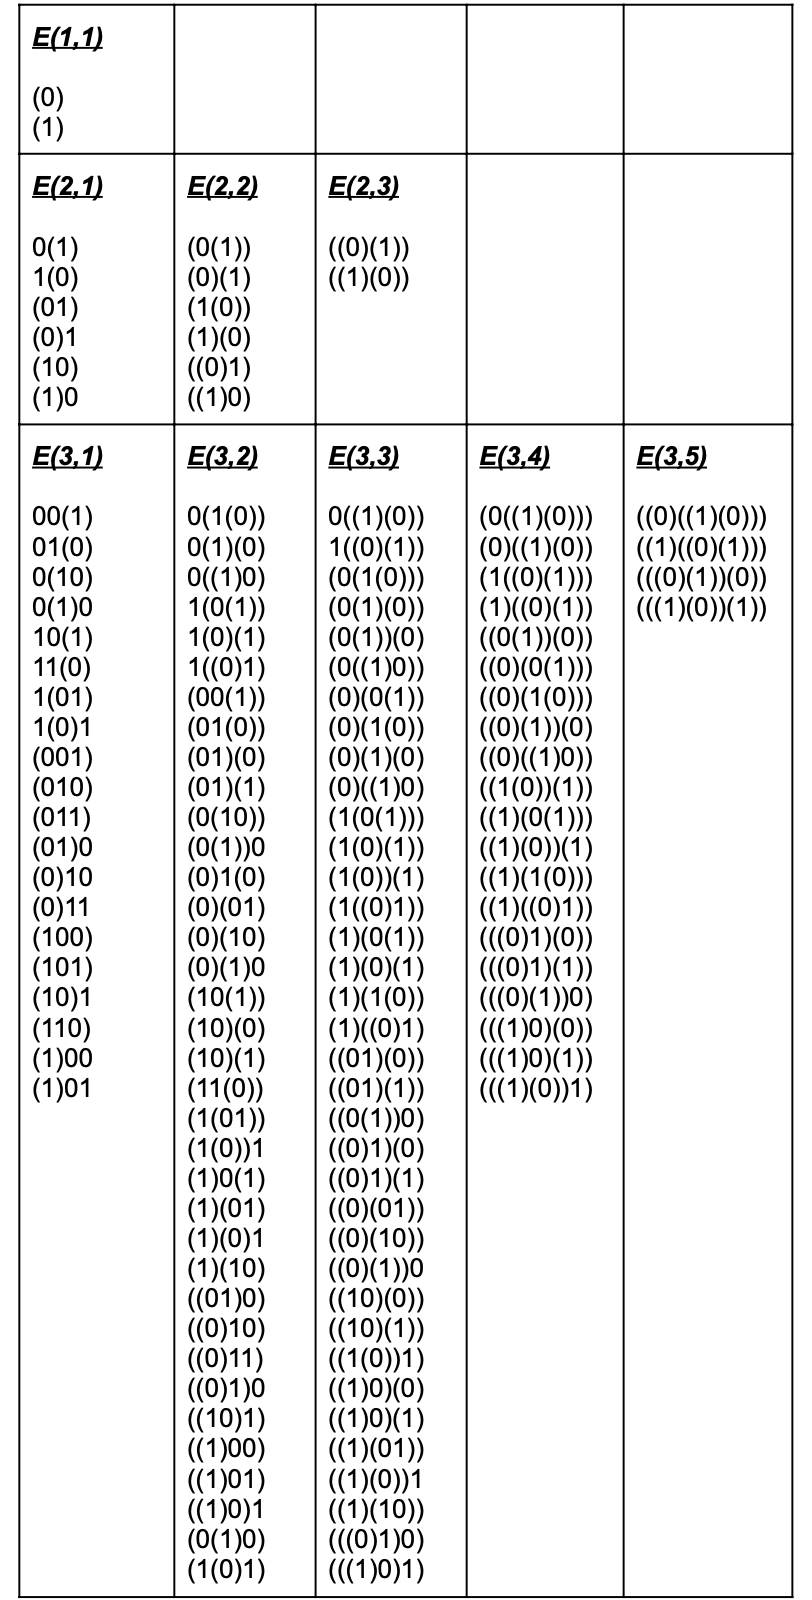
\includegraphics[width=\linewidth]{appendix/sef-seq.png}
    \end{subfigure}
    \caption{Ordered list of equivalence class labels of finite SEFs grouped by length and number of brackets}
    \label{fig:sefseq}
  \end{figure}

  \pagebreak
  \subsection{Concatenation of SEFs}
  \begin{figure}[h!]
    \centering
    \begin{subfigure}[b]{1.0\linewidth}
      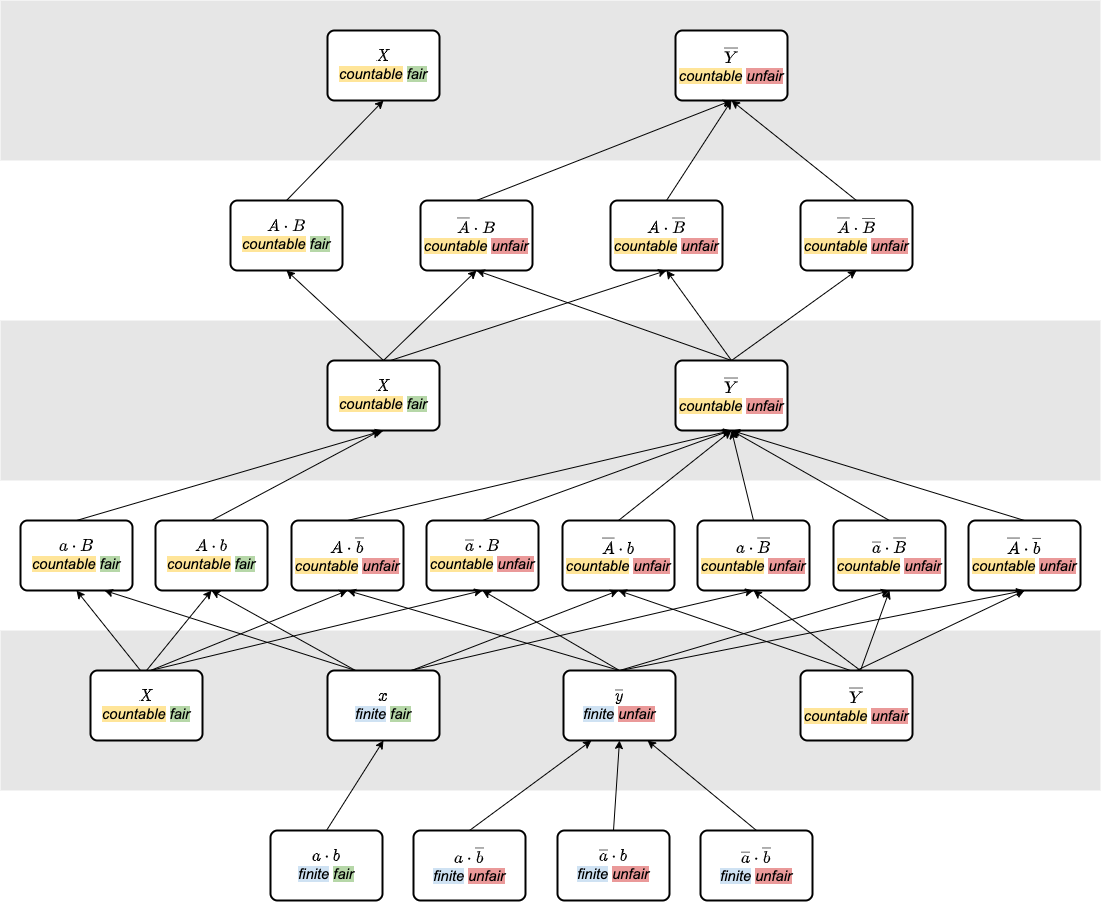
\includegraphics[width=\linewidth]{appendix/concat-hasse-large.png}
    \end{subfigure}
    \caption{Large Hasse-like diagram for SEF concatenation}
    \label{fig:concatlarge}
  \end{figure}

  \pagebreak
  \begin{figure}[h!]
    \centering
    \begin{subfigure}[b]{0.8\linewidth}
      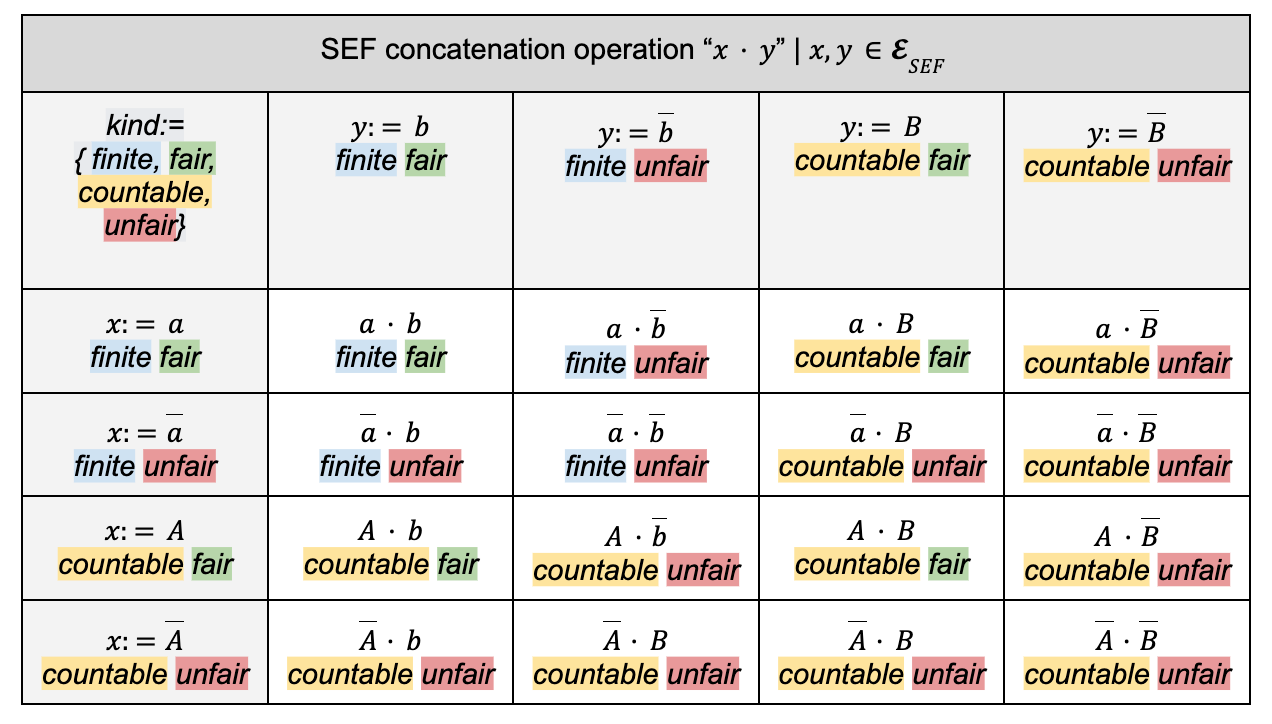
\includegraphics[width=\linewidth]{appendix/concat-table.png}
    \end{subfigure}
    \caption{Table for SEF concatenation operation}
    \label{fig:concattab}
  \end{figure}

  \begin{figure}[h!]
    \centering
    \begin{subfigure}[b]{0.5\linewidth}
      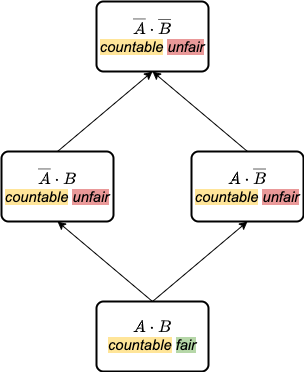
\includegraphics[width=\linewidth]{appendix/concat-hasse-countable.png}
    \end{subfigure}
    \caption{Hasse-like diagram for concatenation of countable SEFs}
    \label{fig:concatcount}
  \end{figure}

  \pagebreak
  \subsection{Power-string operation}
  \begin{figure}[h!]
    \centering
    \begin{subfigure}[b]{0.8\linewidth}
      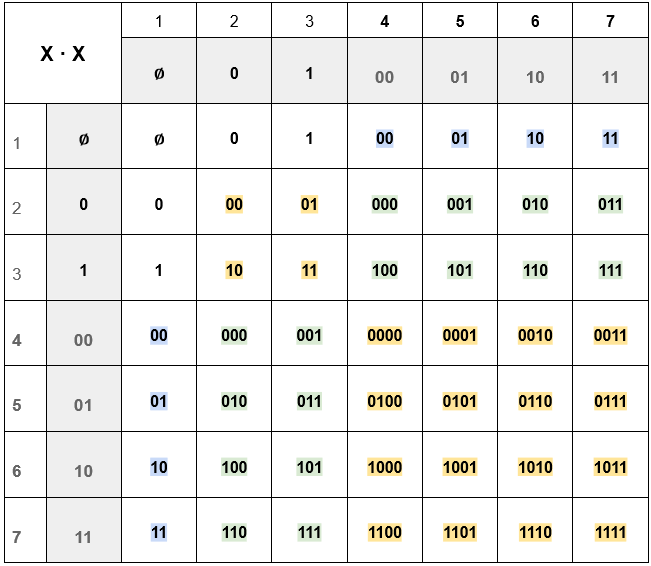
\includegraphics[width=\linewidth]{appendix/power-string.png}
    \end{subfigure}
    \caption{String concatenation table for power-string operation}
    \label{fig:pwrstr}
  \end{figure}

  \begin{table}[ht]
    \caption{Compare power-string and powerset operations}
    \centering
    \begin{tabular}{ |c|r|l| }
      \hline
      \# & power-string $\P(X)$                & powerset $\pset(X)$             \\
      \hline
      0            & $T_0 := \emptyset$        & $V_0 := \emptyset$              \\
      1            & $T_1 := \P(T_0) $         & $V_1 := \pset(V_0)$             \\
      $\dots$      & $\dots $                  & $\dots $                        \\
      $i$          & $T_{i+1} := \P(T_i)$      & $V_{i+1} := \pset(V_{i})$       \\
      \hline
      0            & $|T_0| = 1$               & $|V_0| = 1$                     \\
      1            & $|T_1| = 3$               & $|V_1| = 2$                     \\
      2            & $|T_2| = 7$               & $|V_2| = 4$                     \\
      3            & $|T_3| = 31$              & $|V_3| = 16$                    \\
      4            & $|T_4| = 511$             & $|V_4| = 256$                   \\
      5            & $|T_5| = 131071$          & $|V_5| = 65536$                 \\
      6            & $|T_6| = 8589934591$      & $|V_6| = 4294967296$            \\
      $\dots$      & $\dots $                  & $\dots $                        \\
      $i>0$        & $|T_i| = 2^{2^{i}} - 1$ & $|V_i| = 2^{2^{i-1}}$             \\
      $\dots$      & $\dots $                  & $\dots $                        \\
      \hline
    \end{tabular}
    \label{Tab:PwrStrVsSet}
  \end{table}
  
  \pagebreak
  \subsection{Power-string example in python}
  \lstinputlisting[language=Python]{appendix/pwr-str.py}

  \pagebreak
  \subsection{Set versus String operations}

  \begin{table}[ht]
    \caption{Compare set and string operations}
    \centering
    \begin{tabular}{ |c|c|c| }
      \hline
      \thead{\textbf{set operations}}                                            &  \thead{\textbf{comment}} & \thead{\textbf{string operations}}             \\
      \hline
      \makecell{\\ $x$ is a \textit{member of} $y$: \\ $x \in y$ \\}      &  {\scriptsize is equivalent to} & \makecell{\\ $x$ is a \textit{substring of} $y$: \\ $x \substr y$ \\}   \\
      \hline
      \makecell{\\$y$ is a \textit{subset of} $z$: \\ $y \subset z$ \\ {\tiny or equivalently} \\ $\forall x . [ x \in y \implies x \in z]$ \\}      & {\scriptsize is equivalent to} & \makecell{\\ $y$ is \textit{included in} $z$: \\ $y \Subset  z$ \\ {\tiny or equivalently} \\ $\forall x . [ x \substr y \implies x \substr z]$ \\ {\tiny or equivalently} \\ $\forall x . [ x \in \S(y) \implies x \in \S(z)]$ \\}   \\
      \hline
      \makecell{\\ $s$ is a \textit{union of} $c$: \\ $s = \bigcup c$ \\}  &  \makecell{\\ {\scriptsize \textit{set union}} \\ {\scriptsize is equivalent to} \\ {\scriptsize \textit{class of strings union},} \\ {\scriptsize but not to the \textit{join} which is} \\ {\scriptsize the opposite of \textit{split}} \\} &  \makecell{\\ $[j]$ is a \textit{join of} $z$: \\ $[j] = \mathbb{J}_{s_1, s_2} z$ \\ {\tiny or equivalently} \\ $[j]$ is an equivalence class, s.t. $\forall j \in [j]:$ \\ $\forall x,y . [ x,y \in \S_{s_2}(z) \implies x \cdot s_1 \cdot y \substr j ]$,\\ where $s_1, s_2 \in \Upsilon$ are separators \\}   \\
      \hline
      \makecell{\\$y$ is a \textit{powerset of} $x$: \\ $y = \pset(x)$ \\} & {\scriptsize is equivalent to} & \makecell{\\ $y$ is a \textit{power-string of} $x$: \\ $y = \P(x)$ \\}   \\
      \hline
    \end{tabular}
    \label{Tab:CmpSetVsStrOps}
  \end{table}

  \pagebreak
  \subsection{Examples of recursive Kuratowski notation}

  Given the recursive version of the Kuratowski notation as provided in \textit{Definition \ref{def_kuratowski_morph}}, let us illustrate how it encodes string concatenation to represent strings as sets.

  \begin{table}[ht]
    \caption{String concatenation encoded as sets}
    \centering
    \begin{tabular}{ |c|c|c| }
      \hline
      \thead{\textbf{Tuple/String}} & \thead{\textbf{Tuple/String Encoding}} & \thead{\textbf{Kuratowski Notation}} \\
      \hline
      x = (a,b) & "ab" & $\{\{a\}, \{a, b\}\}$ \\
      y = (c,d) & "cd" & $\{\{c\}, \{c, d\}\}$ \\
      z = x$\cdot$y & "abcd" & \makecell{$\{\{\{\{a\}, \{a, b\}\}, \{c\}\}$, \\ $\{\{\{a\}, \{a, b\}\}, \{c\}\}, d\}\}$ } \\
      \hline
    \end{tabular}
    \label{Tab:ExmplRecKurMorph}
  \end{table}

  Again, note that the complexity of the notation for $\bos abcd \eos$ arises from the recursive structure of the \textit{Definition \ref{def_kuratowski_morph}}. The more elements in the sequence, the more nested the notation becomes.

  \pagebreak
  \subsection{Acknowledgements}

  Significant part of the paper is written in informal style \footnote{including a lot of footnotes and references for non-specialists} with genuine intention to make the discussion a bit more accessible to the wider audience. The disadvantage of this approach is that it often comes at cost of discussing trivialities or even lack of expected rigor in claims. So all of this obviously needs further careful verification and improvement to avoid any potential confusion\footnote{please expect version updates of this paper}. However, author firmly believes that all the presented results are overall correct and will contribute to novel developments in the respective fields.

  Much love, credit and gratitude goes to all cited sources which have been both inspiring and insightful. This also includes many kinds of online discussion forums and resources on mathematics such as wikipedia and youtube, that have not been cited well enough. Special thanks to the communities of math.stackexchange and mathoverflow forums with all the helpful posts on basic results in Set Theory. 

  Finally, sincere sense of gratitude goes to a transitive set of all mathematicians - dead, living or future ones. Author wants to thank the audience for their patience. Comments or remarks are welcomed per email correspondence.

\end{appendices}
